\documentclass{article}\usepackage[]{graphicx}\usepackage[]{color}
%% maxwidth is the original width if it is less than linewidth
%% otherwise use linewidth (to make sure the graphics do not exceed the margin)
\makeatletter
\def\maxwidth{ %
  \ifdim\Gin@nat@width>\linewidth
    \linewidth
  \else
    \Gin@nat@width
  \fi
}
\makeatother

\definecolor{fgcolor}{rgb}{0.345, 0.345, 0.345}
\newcommand{\hlnum}[1]{\textcolor[rgb]{0.686,0.059,0.569}{#1}}%
\newcommand{\hlstr}[1]{\textcolor[rgb]{0.192,0.494,0.8}{#1}}%
\newcommand{\hlcom}[1]{\textcolor[rgb]{0.678,0.584,0.686}{\textit{#1}}}%
\newcommand{\hlopt}[1]{\textcolor[rgb]{0,0,0}{#1}}%
\newcommand{\hlstd}[1]{\textcolor[rgb]{0.345,0.345,0.345}{#1}}%
\newcommand{\hlkwa}[1]{\textcolor[rgb]{0.161,0.373,0.58}{\textbf{#1}}}%
\newcommand{\hlkwb}[1]{\textcolor[rgb]{0.69,0.353,0.396}{#1}}%
\newcommand{\hlkwc}[1]{\textcolor[rgb]{0.333,0.667,0.333}{#1}}%
\newcommand{\hlkwd}[1]{\textcolor[rgb]{0.737,0.353,0.396}{\textbf{#1}}}%
\let\hlipl\hlkwb

\usepackage{framed}
\makeatletter
\newenvironment{kframe}{%
 \def\at@end@of@kframe{}%
 \ifinner\ifhmode%
  \def\at@end@of@kframe{\end{minipage}}%
  \begin{minipage}{\columnwidth}%
 \fi\fi%
 \def\FrameCommand##1{\hskip\@totalleftmargin \hskip-\fboxsep
 \colorbox{shadecolor}{##1}\hskip-\fboxsep
     % There is no \\@totalrightmargin, so:
     \hskip-\linewidth \hskip-\@totalleftmargin \hskip\columnwidth}%
 \MakeFramed {\advance\hsize-\width
   \@totalleftmargin\z@ \linewidth\hsize
   \@setminipage}}%
 {\par\unskip\endMakeFramed%
 \at@end@of@kframe}
\makeatother

\definecolor{shadecolor}{rgb}{.97, .97, .97}
\definecolor{messagecolor}{rgb}{0, 0, 0}
\definecolor{warningcolor}{rgb}{1, 0, 1}
\definecolor{errorcolor}{rgb}{1, 0, 0}
\newenvironment{knitrout}{}{} % an empty environment to be redefined in TeX

\usepackage{alltt}
\usepackage[letterpaper, total={6in, 8in}]{geometry} %size of paper
\usepackage{indentfirst} %indent after section 
\usepackage{graphicx}
\usepackage{amsmath} %number figure based on subsection also
\numberwithin{figure}{subsection} %number figure based on subsection also
\numberwithin{table}{subsection} %number table based on subsection also
\usepackage{booktabs,multirow}%for big bracket
\usepackage{caption}
\captionsetup[figure]{labelfont=bf}
\captionsetup[table]{labelfont=bf,position=below}

\setlength{\parindent}{8ex}
\setlength{\parskip}{2em}
\renewcommand{\baselinestretch}{2.0}
%%%%%%%%%%%%%%%%%%%%%%%%%%%%%%%%%%%%%%%%%%%%%%%%%%%%%%%%%
\IfFileExists{upquote.sty}{\usepackage{upquote}}{}
\begin{document}

\setcounter{section}{6}
\setcounter{page}{28}

\section{Results}
\subsection{Hypothesis Tests}









We found that the difference in Area, Perimeter, Circularity between locations is statistically significant at $0.05$ significance level, as seen in Table~\ref{tab} regardless of which estimators. For the Aspect Ratio, there is not a statistically significant difference between locations. 

Also, we did pairwise comparison tests by using Bonferroni's Correction to correct the significance level of each paired comparison to be $\frac{\text{significance level for Overall Hypothesis Test}}{\text{number of pairwise comparison}} = 0.05/3 \doteq 0.0167$. Hence, as we can be seen in Table~\ref{tab}, we have enough evidence to say mean Area and Perimeter of mitochondria is significantly different between Middle and Distal end and between Proximal and Distal end. The results from the parametric estimators (MLE and 2TAE) is consistent to the nonparametric estimator (Weighted mean) in this case. For Circularity, we only have enough evidence to reject the null hypothesis that mean Circularity of mitochondria at Middle is equal to at Distal.

\bigbreak
%latex.default(tab, rowname = NULL, file = "", n.rgroup = c(2,     2, 1, 1), label = "tab", col.just = c("c", "c", "r", "r",     "r", "r"), caption.loc = c("bottom"), caption = "Unadjusted p-values from Overall and Pairwise Comparison Hypothesis Tests. The significance level for Overall Hypothesis Test is 0.05 and the significance level for Pairwise Hypothesis Test with the Bonferroni correction 0.0167.",     where = "!htbp")%
\begin{table}[!htbp]
\begin{center}
\begin{tabular}{ccrrrr}
\hline\hline
\multicolumn{1}{c}{Property}&\multicolumn{1}{c}{Estimator}&\multicolumn{1}{c}{Overall}&\multicolumn{1}{c}{P vs. M}&\multicolumn{1}{c}{M vs. D}&\multicolumn{1}{c}{P vs. D}\tabularnewline
\hline

Area&WM&\textless 0.0001&0.0974&\textless 0.0001&0.0022\tabularnewline
&MLE&0.0001&0.0950&0.0002&0.0140\tabularnewline
\hline

Perimeter&WM&0.0001&0.2744&\textless 0.0001&0.0018\tabularnewline
&2TAE&\textless 0.0001&0.1518&\textless 0.0001&0.0024\tabularnewline
\hline

Circularity&AM&0.0070&0.2476&0.0022&0.0616\tabularnewline
\hline

Aspect Ratio&AM&0.1838&0.1046&0.1102&0.9884\tabularnewline
\hline
\end{tabular}
\caption{Unadjusted p-values from Overall and Pairwise Comparison Hypothesis Tests. The significance level for Overall Hypothesis Test is 0.05 and the significance level for Pairwise Hypothesis Test with the Bonferroni correction 0.0167.\label{tab}}\end{center}
\end{table}


\newpage
\subsection{Confidence Intervals}








By using Bootstrapping, we found the 95\% confidence interval of the mean by different Locations (Table~\ref{tab_est}). Also, the 98.33\% simultaneous confidence interval of mean differences for each pair which was shown in Table~\ref{tab_ci}. The value 98.33\% is because of the corrected significant value of 0.0167 from Bonferroni's Correction. 




%latex.default(tab_est, file = "", n.rgroup = c(6, 6, 3, 3), label = "tab_est",     col.just = c("c", "c", "c", "r", "r", "r"), caption.loc = c("bottom"),     caption = "Estimate for all mean Properties by Locations and their 95\\% Confidence Interval.",     where = "!htbp")%
\begin{table}[!htbp]
\begin{center}
\begin{tabular}{cccrrr}
\hline\hline
\multicolumn{1}{c}{Property}&\multicolumn{1}{c}{Estimator}&\multicolumn{1}{c}{Location}&\multicolumn{1}{c}{Estimate}&\multicolumn{1}{c}{Lower Bound}&\multicolumn{1}{c}{Upper Bound}\tabularnewline
\hline

Area&WM&Proximal&1928.23&1680.97&2243.38\tabularnewline
&&Middle&2381.80&2038.77&2791.91\tabularnewline
&&Distal&1071.75&873.02&1350.56\tabularnewline
&MLE&Proximal&1221.59&1032.41&1426.77\tabularnewline
&&Middle&1478.75&1276.53&1686.79\tabularnewline
&&Distal&848.79&669.24&1055.76\tabularnewline
\hline

Perimeter&WM&Proximal&176.56&164.50&191.47\tabularnewline
&&Middle&192.90&177.86&209.65\tabularnewline
&&Distal&133.49&121.05&150.04\tabularnewline
&2TAE&Proximal&134.44&123.37&147.17\tabularnewline
&&Middle&147.95&137.35&158.80\tabularnewline
&&Distal&107.26&95.12&120.94\tabularnewline
\hline

Circularity&AM&Proximal&0.744&0.711&0.776\tabularnewline
&&Middle&0.771&0.747&0.794\tabularnewline
&&Distal&0.702&0.668&0.732\tabularnewline
\hline

Aspect Ratio&AM&Proximal&1.529&1.384&1.705\tabularnewline
&&Middle&1.369&1.269&1.490\tabularnewline
&&Distal&1.525&1.409&1.657\tabularnewline
\hline
\end{tabular}
\caption{Estimate for all mean Properties by Locations and their 95\% Confidence Interval.\label{tab_est}}\end{center}
\end{table}


\begin{figure}[!htbp]
  \centering
\begin{knitrout}
\definecolor{shadecolor}{rgb}{0.969, 0.969, 0.969}\color{fgcolor}
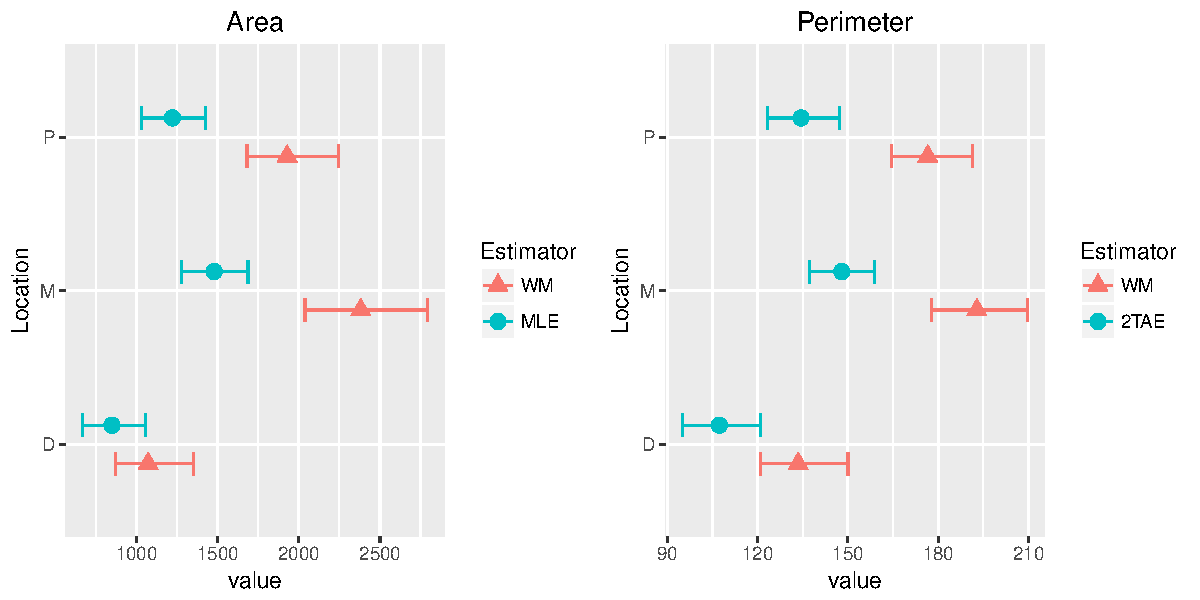
\includegraphics[width=\maxwidth]{figure/unnamed-chunk-13-1} 

\end{knitrout}
  \caption{95\% Confidence Interval for Population Mean Area and Perimeter by Locations.}
  \label{m_area_per}
\end{figure}
\vspace{0.5cm}

\begin{figure}[!htbp]
  \centering
\begin{knitrout}
\definecolor{shadecolor}{rgb}{0.969, 0.969, 0.969}\color{fgcolor}
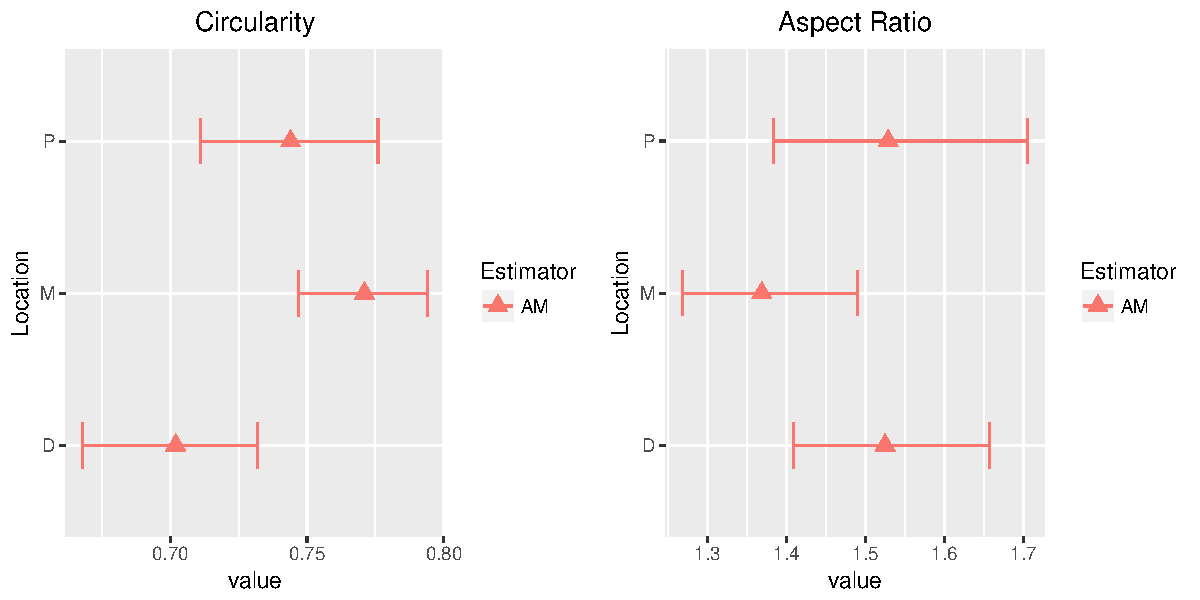
\includegraphics[width=\maxwidth]{figure/unnamed-chunk-14-1} 

\end{knitrout}
  \caption{95\% Confidence Interval for Population Mean Circularity and Aspect Ratio by Locations.}
  \label{m_cir_ar}
\end{figure}
\vspace{0.5cm}

%latex.default(tab_ci, file = "", n.rgroup = c(6, 6, 3, 3), label = "tab_ci",     col.just = c("c", "c", "c", "r", "r", "r"), caption.loc = c("bottom"),     caption = "Estimate for mean Difference and their 98.33\\% Simultaneous Confidence Interval.",     where = "!htbp")%
\begin{table}[!htbp]
\begin{center}
\begin{tabular}{cccrrr}
\hline\hline
\multicolumn{1}{c}{Property}&\multicolumn{1}{c}{Estimator}&\multicolumn{1}{c}{Comparison}&\multicolumn{1}{c}{Difference}&\multicolumn{1}{c}{Lower Bound}&\multicolumn{1}{c}{Upper Bound}\tabularnewline
\hline

Area&WM&P vs. M&-453.57&-1036.89&120.93\tabularnewline
&&M vs. D&1310.06&767.22&1869.39\tabularnewline
&&P vs. D&856.48&400.39&1313.66\tabularnewline
&MLE&P vs. M&-257.16&-602.74&104.31\tabularnewline
&&M vs. D&629.96&274.51&961.36\tabularnewline
&&P vs. D&372.80&27.93&711.49\tabularnewline
\hline

Perimeter&WM&P vs. M&-16.33&-41.63&10.16\tabularnewline
&&M vs. D&59.41&32.03&84.53\tabularnewline
&&P vs. D&43.07&17.92&66.72\tabularnewline
&2TAE&P vs. M&-13.51&-32.27&6.95\tabularnewline
&&M vs. D&40.69&19.23&60.70\tabularnewline
&&P vs. D&27.18&6.09&48.09\tabularnewline
\hline

Circularity&AM&P vs. M&-0.026&-0.077&0.023\tabularnewline
&&M vs. D&0.069&0.020&0.119\tabularnewline
&&P vs. D&0.042&-0.014&0.099\tabularnewline
\hline

Aspect Ratio&AM&P vs. M&0.160&-0.077&0.408\tabularnewline
&&M vs. D&-0.156&-0.360&0.044\tabularnewline
&&P vs. D&0.004&-0.238&0.261\tabularnewline
\hline
\end{tabular}
\caption{Estimate for mean Difference and their 98.33\% Simultaneous Confidence Interval.\label{tab_ci}}\end{center}
\end{table}


\begin{figure}[!htbp]
  \centering
\begin{knitrout}
\definecolor{shadecolor}{rgb}{0.969, 0.969, 0.969}\color{fgcolor}
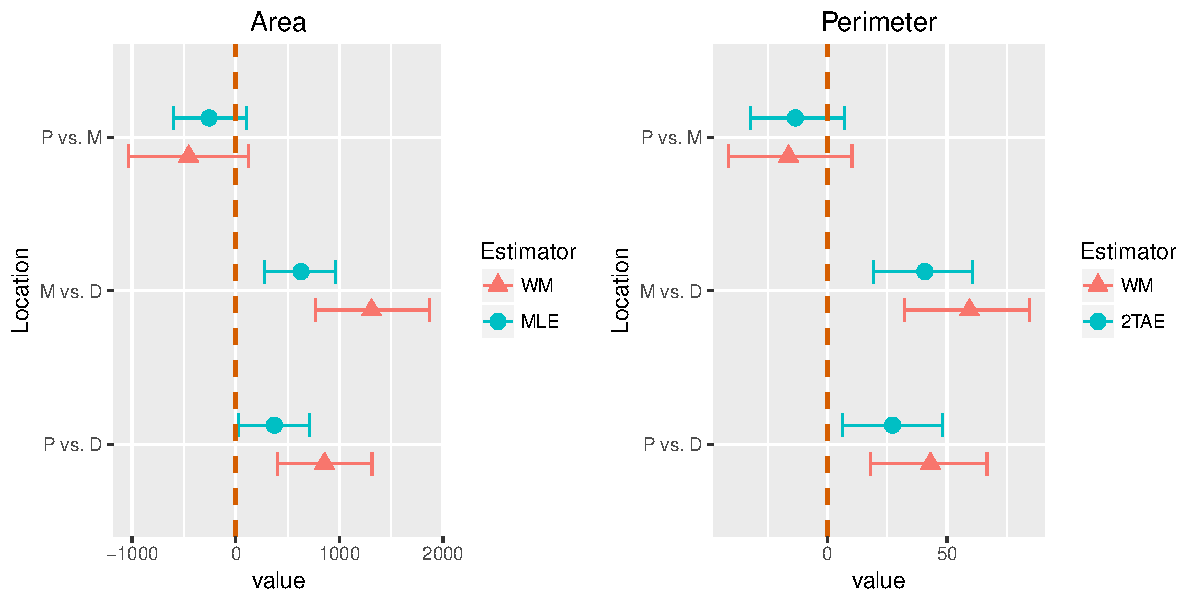
\includegraphics[width=\maxwidth]{figure/unnamed-chunk-16-1} 

\end{knitrout}
  \caption{98.33\% Confidence Interval for mean Difference by Locations for Area and Perimeter.}
  \label{m_area_per_diff}
\end{figure}
\vspace{0.5cm}

\begin{figure}[!htbp]
  \centering
\begin{knitrout}
\definecolor{shadecolor}{rgb}{0.969, 0.969, 0.969}\color{fgcolor}
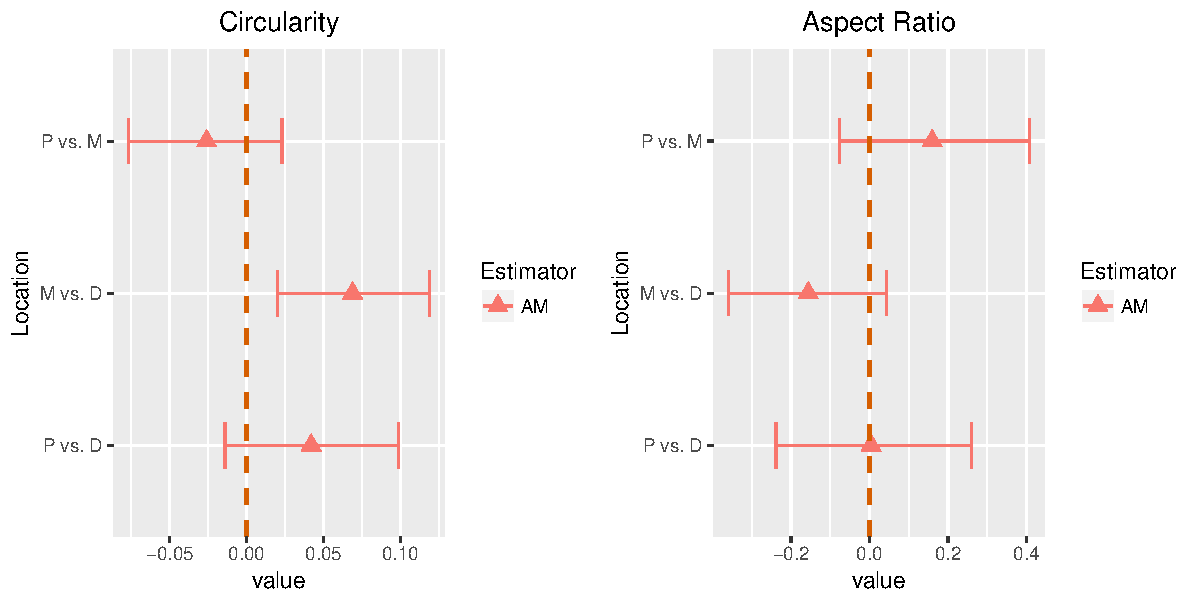
\includegraphics[width=\maxwidth]{figure/unnamed-chunk-17-1} 

\end{knitrout}
  \caption{98.33\% Confidence Interval for mean Difference by Locations for Circularity and Aspect Ratio.}
  \label{m_cir_ar_diff}
\end{figure}
\vspace{0.5cm}

\end{document}
